\documentclass[twoside,colorbacktitle,accentcolor=tud1b]{tudexercise}
\usepackage[english]{babel}
\usepackage[export]{adjustbox}
%\usepackage{subfig}
\usepackage{subcaption}

\newcommand{\unit}[1]{{\rm\,#1}}

\title{Submission for Milestone 1
\linebreak[1] Middleware Project
\linebreak[1] Winter Term 2014/15}
\subtitle{Manisha Luthra (2687667) \\
Patrick Welzel (1478819)\\
Pratyush Agnihotri (2387187)}
%\subsubtitle{"Ubungsblatt \arabic{section}}


\begin{document}
  \begin{examheader}
    \textmb{Submission for Milestone 1
	\linebreak[1] by: Patrick Welzel (1478819)
      Manisha Luthra (2687667)
      Pratyush Agnihotri (2387187)}
  %  \examheaderdefault
  \end{examheader}
\setcounter{section}{1}
\maketitle
  \subsection{Goal overview}
  In this milestone, we achieved to design an overall architecture for the project with all the entities, attributes and relationship between the entities in place. Furthermore, we completed the first module implementation i.e. Customer and Product Data Management. In the following sections we discuss the architectural details and the implementation logic in detail.
  \subsection{Architectural overview}
After thoroughly understanding the requirements given for the project, we derived the entities: $Customer$, $Product$, $Employee$, $Order$, $Shipment$, $Truck$ and $Event$ and their corresponding attributes. In the following table (Table I) we have illustrated on the entities and their attributes, (the underlined) primary key and (asterisk* mark) foreign keys we will refer to in the code.
\begin{table}[htbp]
  \centering
  \caption{Entities and attributes}
  	\begin{tabular}{|c|c|c|}
	\hline
	\textbf{Entity} & \textbf{Attribute} \\
	\hline
	Customer & \underline{customerId}, customerName,\\
	 & customerAddress, customerEmailId \\	
	\hline
	Product & \underline{productId}, productName, productPrice \\
	\hline
	Employee & \underline{employeeId}, employeeName \\
	\hline
	Order & \underline{orderId}, orderStatus*, \\
	 & orderQty, orderCost \\
	\hline
	Shipment & \underline{shipmentId}, orderStatus*, \\
	 & shipmentCost, shipmentPos*, excDesc* \\
	\hline
	Truck & \underline{truckId}, shipmentPos* \\
	 & (latitude \& longitude value), truckCapacity \\
	 & (in no of shipments) \\
	\hline
	Event & \underline{eventId}, eventType, \\
	 & excDesc*, eventSrc \\
	\hline
	\end{tabular}%
  \label{tab:addlabel}%
\end{table}%

Next, we defined the relationships between the various entities discussed in the above table and defined the cardinalities between the relation function. The entity relationship diagrams for the entities shown above is illustrated in Fig. 1.

\begin{figure}[h!]
  \centering
   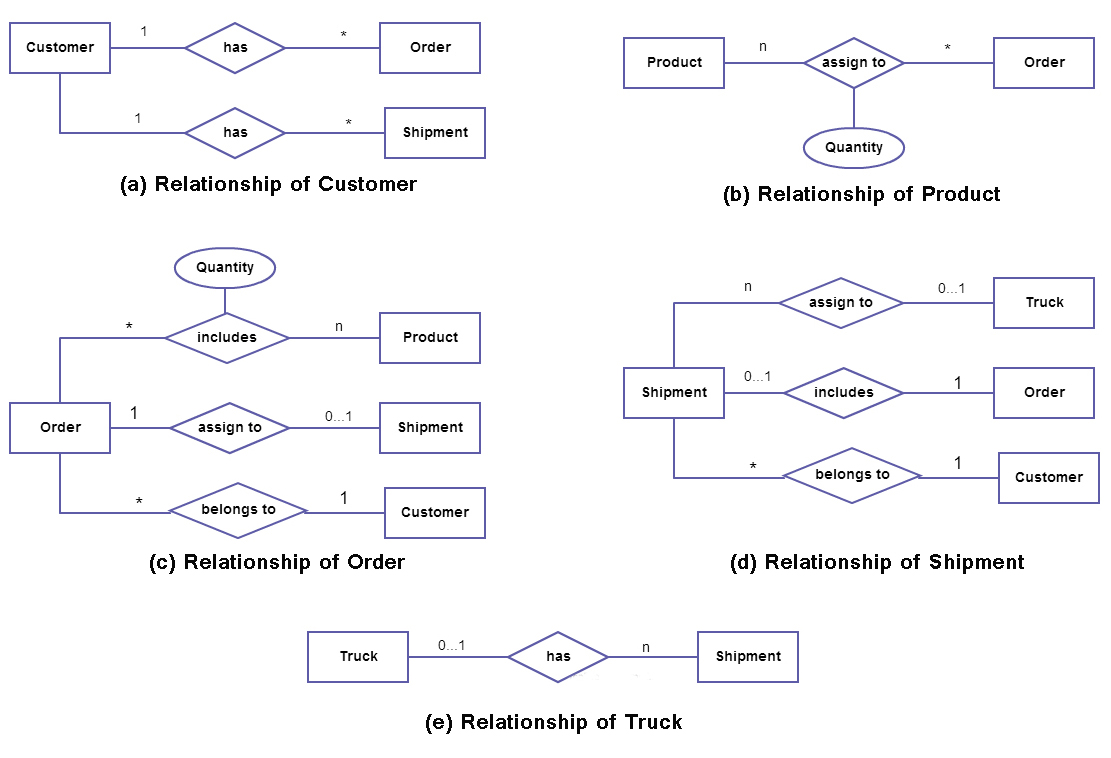
\includegraphics[width=17cm]{associations}
   \caption{ER diagram}
\end{figure}

  \subsection{Encountered problems/Implementation Alternatives}
 \textbf{Complexity of the models :}\\
While designing the architecture for Omazon, we encountered implementation problems such as, mainly how complex our model should be? Should we take into account, how the things should work in general, or just keep it simple and understandable as given in the problem statement. Alternatives that we considered:-\\
1) Go with the way how it should work in general, and consider the usual usage patterns that the system should adopt. For instance, a customer name can have two attributes in general, first name and last name.\\
2) Adapt sticking to the basic things that makes it understandable and usable but not overflow it with too many details. \\
We decided to opt with the second approach, and just conform with the basic things that makes our project understandable. So that, we could draw the attention in understanding the major concepts of Java Enterprise edition - Enterprise Beans, data persistence and work on them.

\begin{figure}[h!]
  \centering
   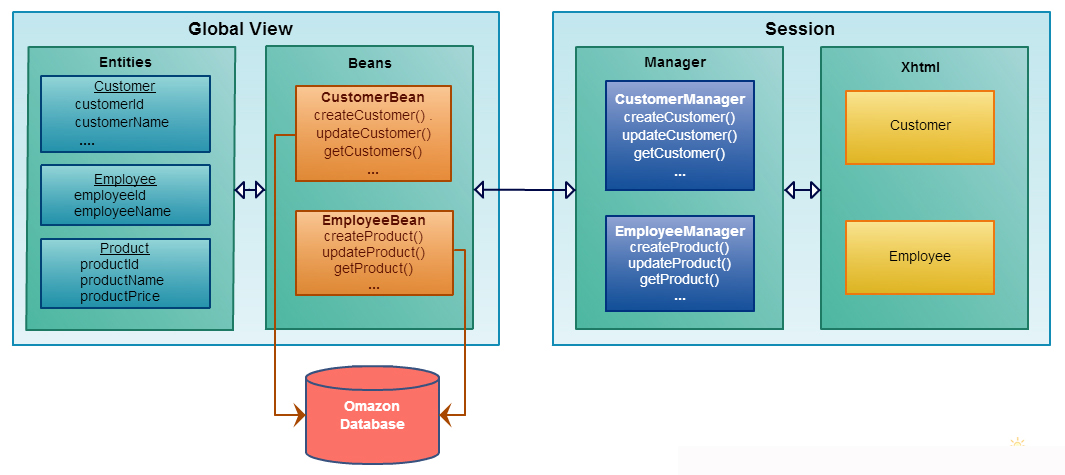
\includegraphics[width=17cm]{BusinessLogic}
   \caption{Business Logic Flow}
\end{figure}
\clearpage
 \subsection{Implemented features}
  We chose NetBeans IDE, Glassfish application server and JDBC for our project. To get familiar with the java enterprise edition, we started with the order example of JavaEE 6 and started building upon this as a base project. We have briefly discussed in the following sections on further implementation. 

\subsubsection{Customer and product data management}

As seen in the architectural overview, the design contains a Customer model representing the customers of Omazon Inc. with its respective properties as seen in Fig. 2.
These properties are grouped together in an entity called $Customer$ together with additional database relevant information eg some queries for this model on the database or its $primary key$ property.
For handling of customers the $CustomerBean$ is created, encapsulating all actions that can be done with the $Customer$ Entity.
This includes creating, updating, loading from the database of all or one specific entity.

The same is done for the $Product$ model representing the product data (done by $EmployeeManager$) and an according $EmployeeBean$.

\subsubsection{User Interface}
The user interface is implemented as a web interface with Java Server Faces(JSF) as seen in Fig. 3.
The logic and data representation of the user interface is split up into Java Server Pages (JSP) written in xhtml and one or more associated $managers$.
In the JSP the direct user interface is defined, mainly which elements the user sees and can interact with and what and how data is presented.
The managers contain the logic of (the part of) the user interface, dealing with optionally displayed elements in certain cases or form inputs.
E.g. the $CustomerManager$ handles the filling of the table showing all customers creation as well as the form for creation and edit of customers.
It redirects respectively triggers the actions to/on the according beans.

While the bean is stateless and contains only how to do things with certain models, the managers have a state and in this case belong to a session of a user.
JSF uses \textit{Dependency Injection} to deal with the differently scoped entities and the creation of the instances when needed.

\begin{figure}[h!]
  \centering
   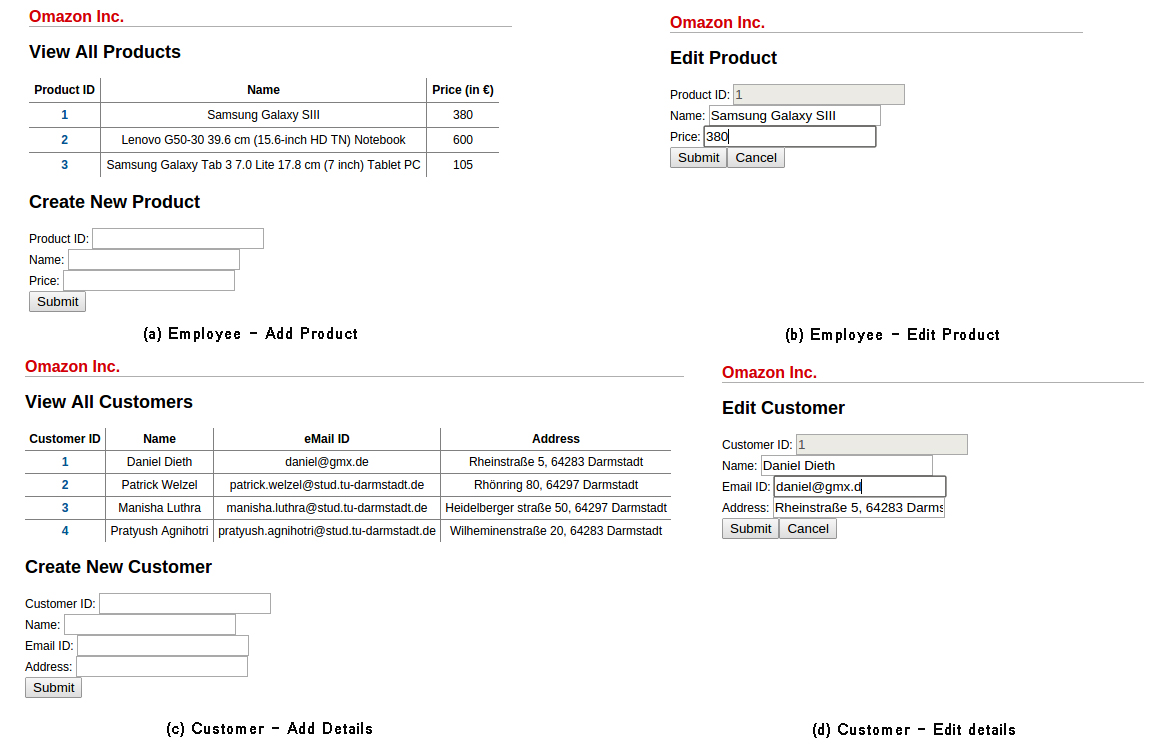
\includegraphics[width=16cm]{GUI}
   \caption{Web interface}
\end{figure}

\end{document}
